% Compile with:  pdflatex heart_stellarator.tex
\documentclass[11pt,a4paper]{article}

\usepackage[a4paper,margin=2.5cm]{geometry}
\usepackage{graphicx}
\usepackage{amsmath}
\usepackage{hyperref}
\usepackage{xcolor}
\usepackage{listings}
\usepackage{parskip}

\hypersetup{
  colorlinks=true,
  urlcolor=blue!60!black,
  linkcolor=black,
}

\lstdefinestyle{py}{
  language=Python,
  basicstyle=\ttfamily\footnotesize,
  keywordstyle=\color{blue!70!black}\bfseries,
  commentstyle=\color{gray!50!black}\itshape,
  stringstyle=\color{red!60!black},
  showstringspaces=false,
  breaklines=true,
  frame=single,
  framerule=0.4pt,
  rulecolor=\color{black!30},
  columns=fullflexible,
}

\title{A Heart-Shaped Stellarator}
\author{}
\date{}

\begin{document}
\maketitle

\section*{Fusion energy in thirty seconds}

When two light nuclei merge into a heavier one, a tiny fraction of their
mass is converted to energy via $E = mc^{2}$. The easiest reaction to
achieve on Earth is
\[
  {}^{2}\mathrm{H} + {}^{3}\mathrm{H}
    \;\longrightarrow\; {}^{4}\mathrm{He} + n + 17.6\,\mathrm{MeV},
\]
deuterium fusing with tritium. To overcome the Coulomb repulsion between
the positively-charged nuclei the fuel must be heated to roughly
$1.5\times 10^{8}\,\mathrm{K}$ --- about ten times hotter than the core
of the Sun. At those temperatures matter is a plasma, and the only known
way to confine it long enough is with magnetic fields, because no material
wall survives contact. The product of density, temperature and confinement
time has to clear the Lawson criterion for net power.

The two practical magnetic geometries are the \emph{tokamak} (axisymmetric,
plasma current induces the rotational transform) and the \emph{stellarator}
(non-axisymmetric, the rotational transform comes from external coils).
Stellarators are harder to design but inherently steady-state and free of
current-driven disruptions.

\section*{The startup hype}

For sixty years magnetic confinement was the province of national labs ---
JET in the UK, TFTR at Princeton, Wendelstein~7-X in Germany, the
multinational ITER now being assembled in France. Around 2015 a new wave
of private companies arrived, betting that high-temperature superconductors
(HTS), modern HPC, and machine-learning-driven design could collapse the
path to a power plant. Commonwealth Fusion Systems raised \$1.8\,B in 2021
for its SPARC tokamak. Helion is targeting a 50\,MW plant for Microsoft.
Tokamak Energy, TAE, Zap, Type One Energy, Proxima Fusion, and others have
together pulled in well over \$7\,B in private capital. The promise is
electricity on the grid by the early 2030s; the risk is that half a dozen
``first-of-a-kind'' demonstrators each need much longer than their plans
assume.

\section*{Codes that design plasmas and coils}

A magnetic-confinement reactor is two coupled design problems. The
\emph{plasma boundary problem} asks: what shape of nested flux surfaces
gives good confinement, low turbulent transport, manageable divertor heat
loads, and MHD stability? The \emph{stage-two coil problem} asks: what set
of external coils will produce that boundary as the outermost flux
surface?

The standard tools, almost all originally written in Fortran in national
labs, are now driven from Python:

\begin{itemize}
  \item \textbf{VMEC} (Hirshman, ORNL, 1983) --- variational 3-D MHD
    equilibrium solver. Still the reference for fixed- and free-boundary
    equilibria.
  \item \textbf{BNORM} and \textbf{NESCOIL} (Merkel, IPP Garching) ---
    compute the normal field from a given coil set, and inversely the
    surface current that would produce a target plasma boundary.
  \item \textbf{STELLOPT} (PPPL/IPP) --- the stellarator-optimization
    driver that wraps VMEC, BNORM, NESCOIL and dozens of physics targets.
  \item \textbf{SIMSOPT} (Landreman \emph{et al.}, 2021) --- a modern
    Python framework with C++/Eigen Biot--Savart kernels that supersedes
    much of STELLOPT's role for coil and shape optimization.
\end{itemize}

In a typical stage-two coil-design run one picks a target plasma boundary
$S$ as a \texttt{SurfaceRZFourier} object, parametrizes the modular coils
as \texttt{CurveXYZFourier} loops, and minimizes
\[
  J \;=\; \tfrac{1}{2}\int_{S}\!\bigl(\mathbf{B}\cdot\hat{\mathbf{n}}\bigr)^{2}\,\mathrm{d}A
     \;\;+\;\; \sum_{i} w_{i}\,P_{i}(\text{coils})
\]
with L-BFGS-B. The first term forces the coil field to be tangent to the
target surface --- so the surface really is a flux surface. The penalty
terms $P_{i}$ keep the coils realistic: bounded length, bounded curvature,
no coil--coil collisions, well-conditioned arc-length parametrization.

\section*{What we built}

The script \texttt{heart\_stellarator.py} designs a stellarator whose
poloidal cross-section is the classical parametric heart curve
\begin{align*}
  x(t) &= 16\sin^{3} t \;=\; 12\sin t - 4\sin 3t, \\
  y(t) &= 13\cos t - 5\cos 2t - 2\cos 3t - \cos 4t.
\end{align*}
This is already a finite Fourier series, so it drops straight into a
\texttt{SurfaceRZFourier} with no fitting --- five $R_{m,0}$ modes and
two $Z_{m,0}$ modes recover the heart exactly. Rotated $90^{\circ}$ in
the $(R, Z)$ plane the curve becomes stellarator-symmetric:
$R(-\theta) = R(\theta)$, $Z(-\theta) = -Z(\theta)$. A small $n=1$
perturbation twists the heart as it goes around the torus, turning a
heart-tokamak into a real, non-axisymmetric, two-field-period stellarator.

Five modular coils per half-period are then initialized as equally spaced
circles and optimized against the heart surface. After 84 L-BFGS-B
iterations the relative normal field $\langle|\mathbf{B}\cdot\hat{\mathbf{n}}|/|\mathbf{B}|\rangle$
drops from $\sim 5\%$ to $1.17\%$, with a mean coil length of $3.15\,\mathrm{m}$.

\begin{lstlisting}[style=py,caption={Core of the heart-stellarator design.}]
s = SurfaceRZFourier(nfp=2, stellsym=True, mpol=5, ntor=2, ...)
s.set_rc(0, 0, R0)
s.set_rc(1, 0,  A * 13.0); s.set_rc(2, 0, -A *  5.0)
s.set_rc(3, 0, -A *  2.0); s.set_rc(4, 0, -A *  1.0)
s.set_zs(1, 0,  A * 12.0); s.set_zs(3, 0, -A *  4.0)
s.set_rc(1, 1,  twist);    s.set_zs(1, 1, -twist)

base_curves = create_equally_spaced_curves(5, s.nfp, stellsym=True, ...)
coils = coils_via_symmetries(base_curves, base_currents, s.nfp, True)
bs = BiotSavart(coils)
JF = SquaredFlux(s, bs) + length_pen + curv_pen + dist_pen
minimize(lambda x: (JF.J(), JF.dJ()), JF.x, jac=True, method="L-BFGS-B")
\end{lstlisting}

The whole pipeline runs in a Docker container that compiles SIMSOPT from
source for the host CPU --- the PyPI \texttt{simsoptpp} wheel uses ARM
instruction-set extensions the lightweight Colima VM does not expose, so
a stock \texttt{pip install simsopt} would crash with an illegal-opcode
trap on first call.

\section*{Result}

\begin{figure}[h!]
  \centering
  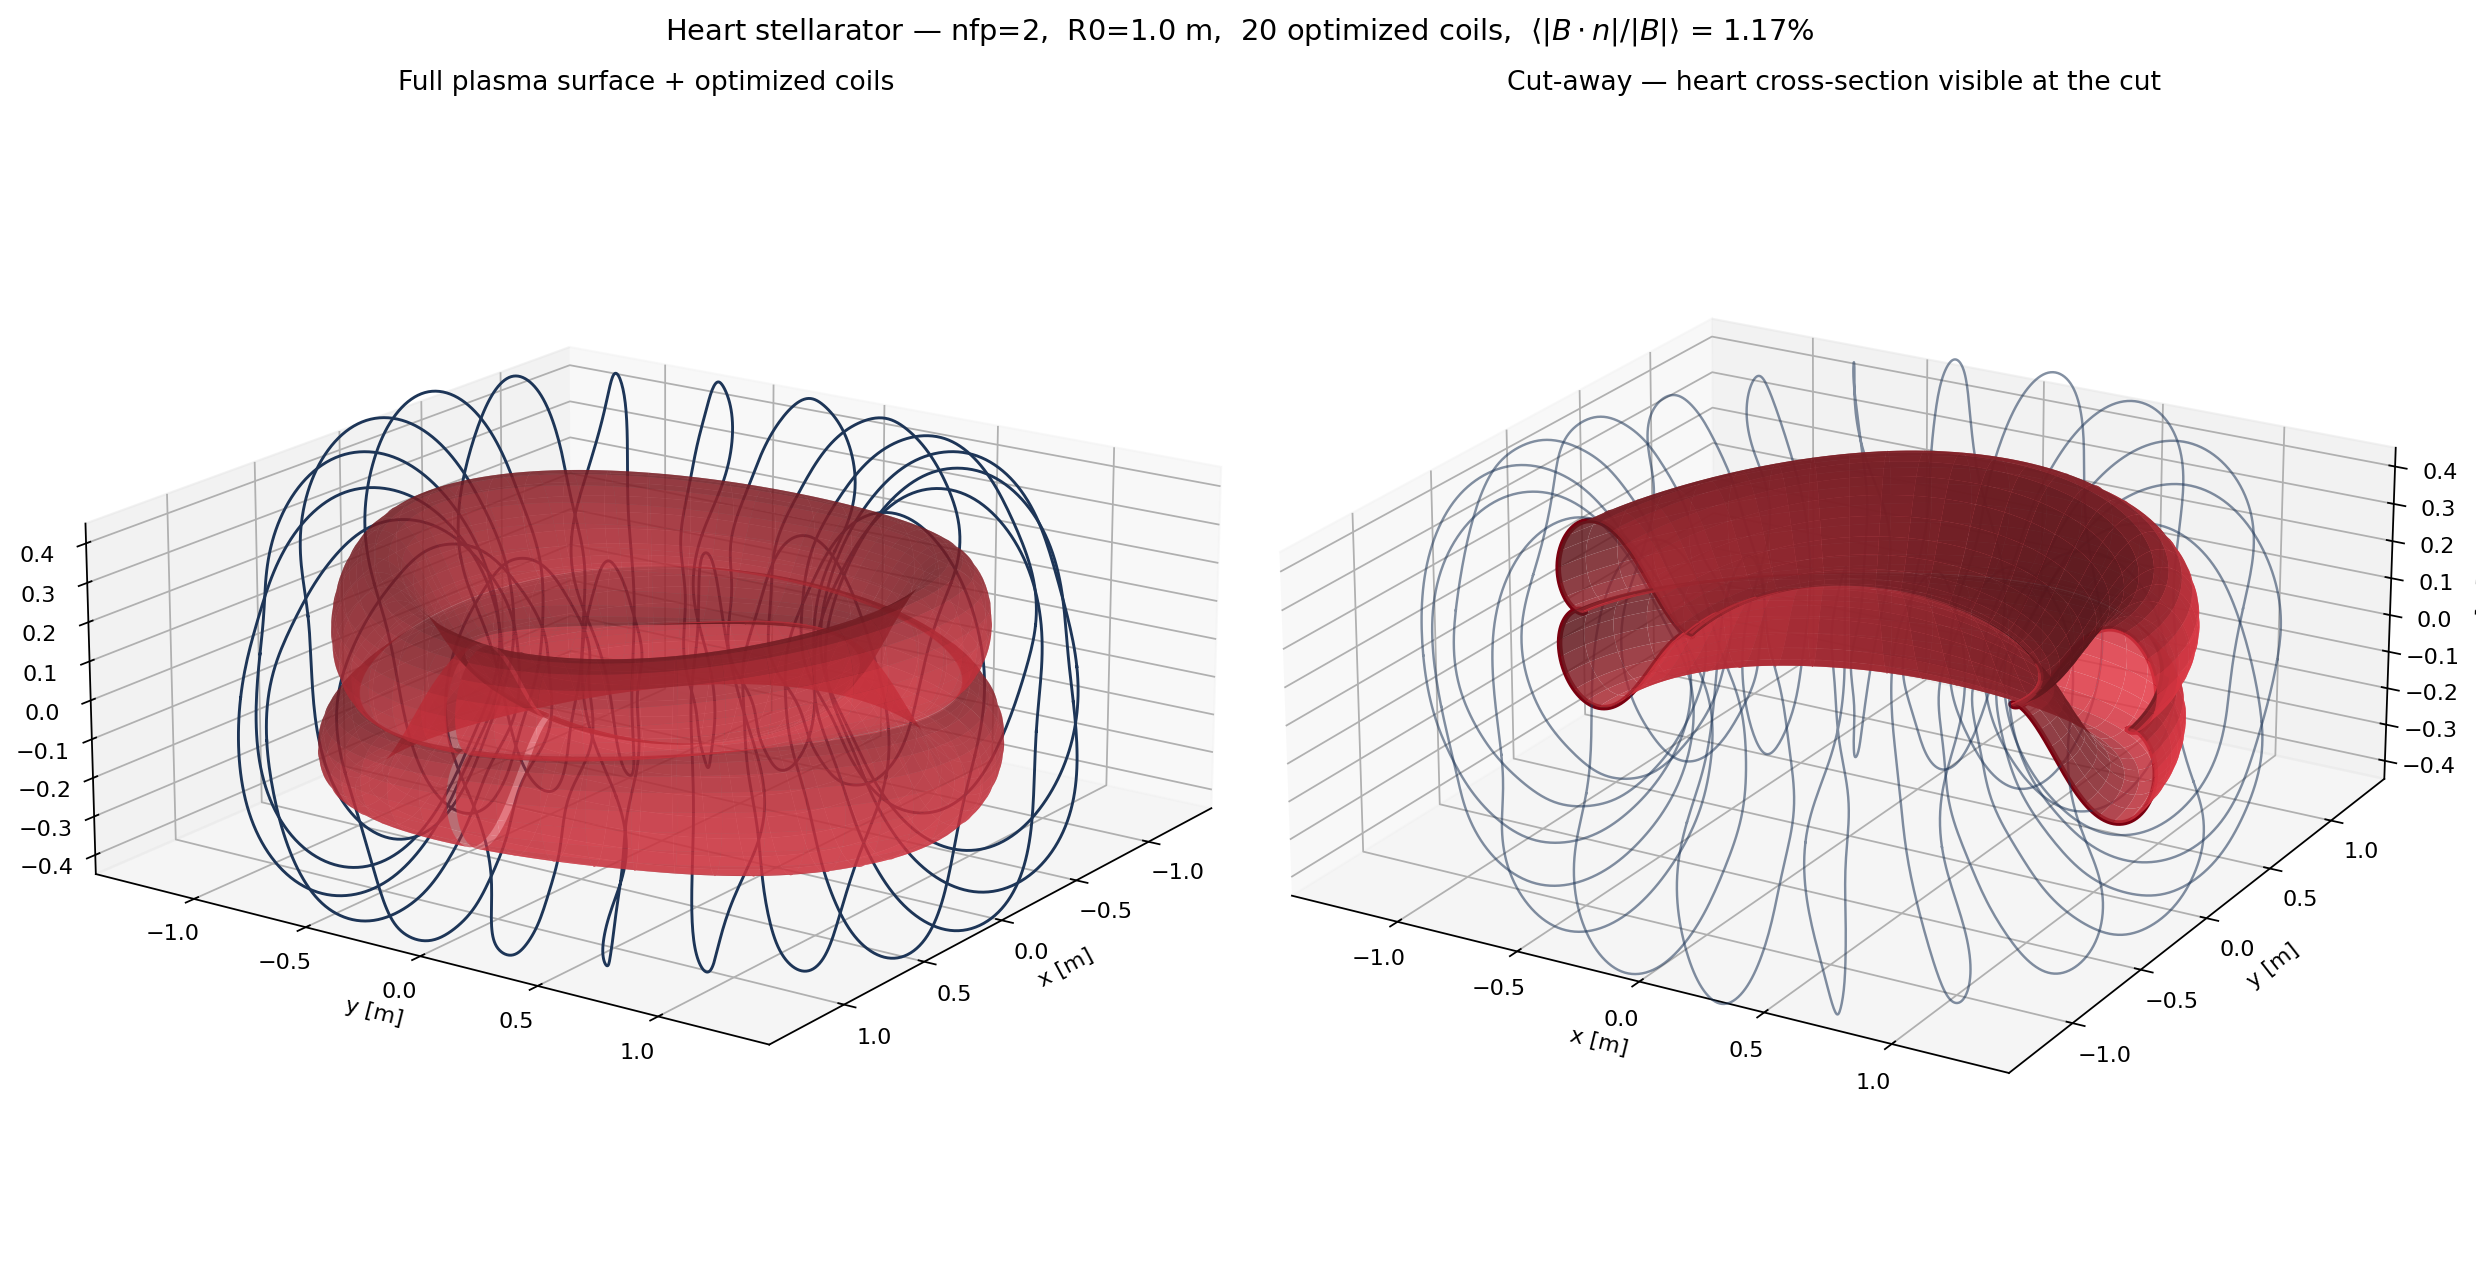
\includegraphics[width=0.98\textwidth]{heart_stellarator.png}
  \caption{The optimized heart stellarator.
    \emph{Left:} the full plasma boundary (red) wrapped by 20 modular
    coils (5 unique $\times$ 2 field periods $\times$ stellarator
    symmetry).
    \emph{Right:} a half-torus cut-away that exposes the heart
    cross-section --- two lobes outboard, a smooth dip between them, a
    tip pointing inboard. The L-BFGS-B optimizer reaches
    $\langle|\mathbf{B}\cdot\hat{\mathbf{n}}|/|\mathbf{B}|\rangle = 1.17\%$.}
  \label{fig:heart}
\end{figure}

\noindent Source code:
\href{https://github.com/GrumpyGoedel/heart-stellarator}{github.com/GrumpyGoedel/heart-stellarator}.

\end{document}
